\subsection{Disponibilidad}
    
Como mencionamos en la introduccion de este capitulo, los conjuntos de datos pueden estar disponibles en la fuente original, pero no por
ello significa que estos sean accesibles.
Los retos a los que nos encontramos con los datos crudos, directos de la fuente de origen, son los siguientes:\\
    
 
\textbf{Localizacion}. Los conjuntos de datos se encuentran disponibles en portales de datos abiertos organizados 
y estructurados, normalmente se necesita una tarea de busqueda y seleccion
a veces complicada. Aunque las empresas ponen cada vez mas de su parte en ofrecer una interfaz 
agradable y funcional a los usuarios, esta tarea requiere de un trabajo de investigacion por parte del usuario,
ya que posiblemente, debera buscar en distintos portales.\\

\textbf{Extraccion}. Los conjuntos de datos suelen estan disponibles a traves de una interfaz de programacion 
de aplicaciones (API) no facilmente interpretable por el usuario medio. Normalmente cuenta con 
un documento que describe cada uno de los campos y valores que se presentan en el documento y como utilizar la API.\\

\textbf{Legibilidad}. Usualmente los conjuntos de datos estan representados en un formato para ser procesado por 
algun software, por lo que su lectura resulta complicada por el usuario medio, en el mejor de los casos, 
estaran representados en una tabla y aun asi, sera muy dificil de extraer informacion. 

Por lo tanto, no podemos decir que estos datos sean accesibles de una forma util para el usuario medio.\\

\subsubsection{How to solve it.} 

Deberemos proporcionar la informacion requerida por el usuario de forma directa, facil de leer e interpretar. En un formato
que sea facil y rapido de asimilar.

Para la correcta utilizacion de de los datos deberemos realizar procesos tales como  la extraccion, transformacion y 
limpieza de los datos, asi se obtienen los datos que se necesitan para mostrar la informacion util. 
 
\subsubsection{How we solve it. Aire Guru.} 

Nuestra herramienta utiliza los datos de calidad del aire proporcionados por el ayuntamiento de Malaga en su portal de datos abiertos.\footnote{\url{https://datosabiertos.malaga.eu/}}\\
\begin{figure}[ht]
    \centering
   \subfigure[Pagina principal]
    {\includegraphics[width=5.5cm  ]{OpenDataPortal}}
    \hfill
    \subfigure [Categoria medio ambiente]
       { 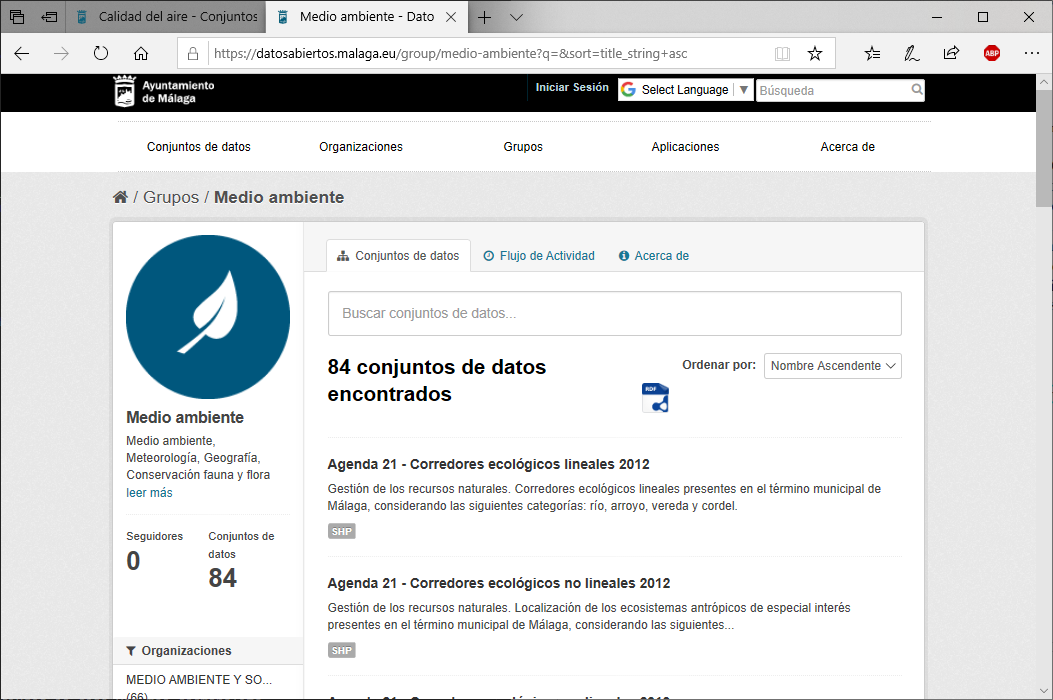
\includegraphics[width=5.5cm]{openDataPortalEnviromentCategory}}
    \vfill
     \subfigure[GeoJson Document]
     { \centering 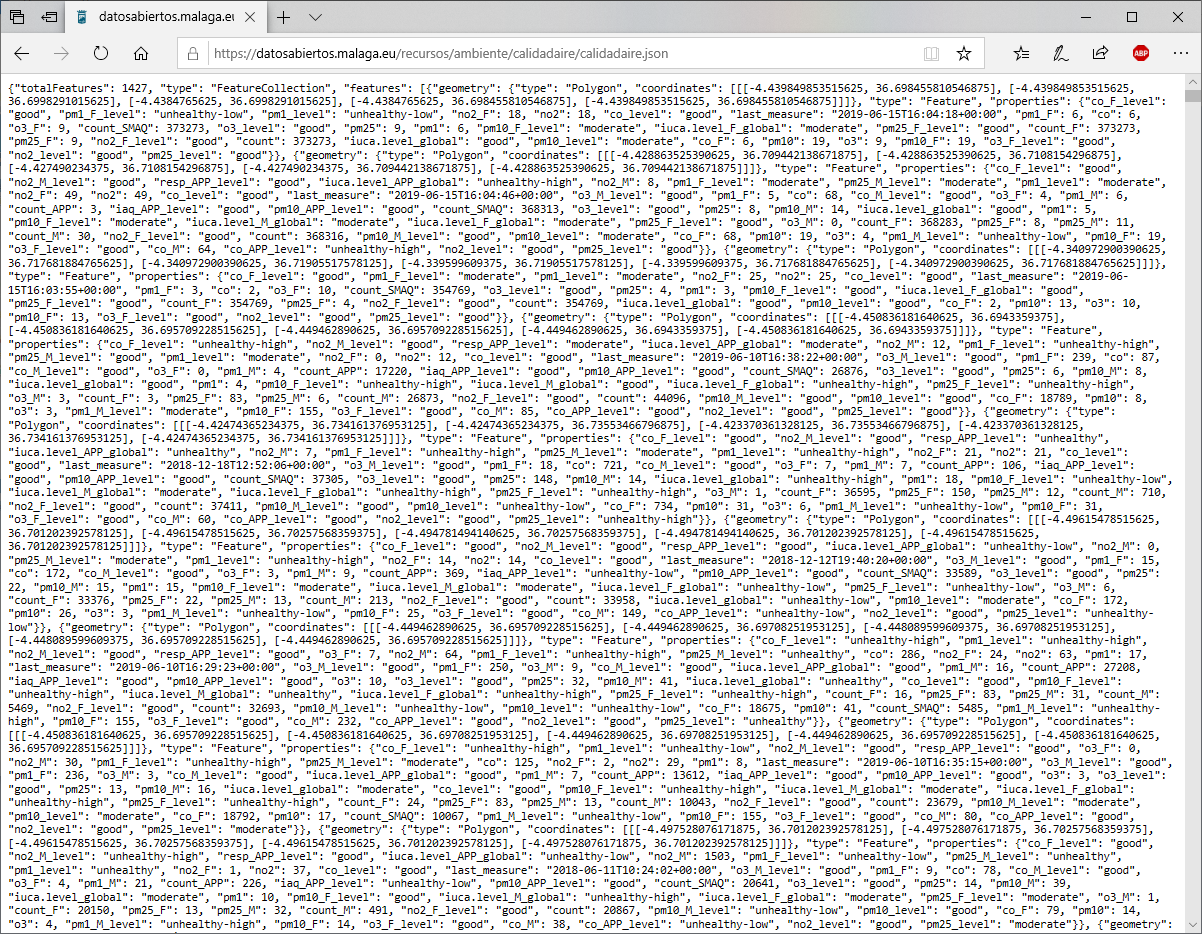
\includegraphics[width=4.75cm]{geoJsonAirQualityDataRaw}}
  
  \caption{Open Data Portal Malaga}
    \end{figure}

    Este portal de datos ofrece una oferta de categorias representados por iconos, por lo que es necesario saber en que categoria se clasifica el conjunto
de datos, una vez que se accede a la categoria, tenemos una barra buscadora que nos permite insertar las palabras claves para buscar el conjunto de datos
deseado.\\

En este caso puede pulsarse sobre el enlace y este abrira los datos en una nueva pestana, por lo que la utilizacion de un sistema informatico
para la descarga de los datos no es extrictamente necesario, pero podemos ver que ver que el formato no es legible, al menos desde el punto
de vista humano. 

AireGuru \footnote{\url{https:\\aire.guru}} ofrece toda la informacion necesaria en una plataforma web con una visualizacion adaptada
a la comprension humana.
\newpage
\elsparagraph{Evaluation}  

\begin{itemize}
    \done Localizacion. La localizacion de los datos es directa, ya que ofrece informacion desde el primer momento en que se accede a la web. En la pagina principal
    presenta los niveles de polucion en todas las zonas sin necesidad de realizar ninguna seleccion.
    \done Extraccion. No es necesario ningun software o conocimientos informaticos para acceder la informacion.
    \done Legibilidad. Contiene un mapa donde los niveles de polucion se presentan por colores. Estos colores estan definidos por una leyenda justo
    debajo del mapa. Cuenta con un glosario donde se explica los conceptos expuesto en la pagina web, el significado de cada seccion y como
    navegar por la pagina web.
 

\end{itemize}
\newpage

 


